\documentclass{beamer}\usepackage[]{graphicx}\usepackage[]{color}
%% maxwidth is the original width if it is less than linewidth
%% otherwise use linewidth (to make sure the graphics do not exceed the margin)
\makeatletter
\def\maxwidth{ %
  \ifdim\Gin@nat@width>\linewidth
    \linewidth
  \else
    \Gin@nat@width
  \fi
}
\makeatother

\definecolor{fgcolor}{rgb}{0.345, 0.345, 0.345}
\newcommand{\hlnum}[1]{\textcolor[rgb]{0.686,0.059,0.569}{#1}}%
\newcommand{\hlstr}[1]{\textcolor[rgb]{0.192,0.494,0.8}{#1}}%
\newcommand{\hlcom}[1]{\textcolor[rgb]{0.678,0.584,0.686}{\textit{#1}}}%
\newcommand{\hlopt}[1]{\textcolor[rgb]{0,0,0}{#1}}%
\newcommand{\hlstd}[1]{\textcolor[rgb]{0.345,0.345,0.345}{#1}}%
\newcommand{\hlkwa}[1]{\textcolor[rgb]{0.161,0.373,0.58}{\textbf{#1}}}%
\newcommand{\hlkwb}[1]{\textcolor[rgb]{0.69,0.353,0.396}{#1}}%
\newcommand{\hlkwc}[1]{\textcolor[rgb]{0.333,0.667,0.333}{#1}}%
\newcommand{\hlkwd}[1]{\textcolor[rgb]{0.737,0.353,0.396}{\textbf{#1}}}%

\usepackage{framed}
\makeatletter
\newenvironment{kframe}{%
 \def\at@end@of@kframe{}%
 \ifinner\ifhmode%
  \def\at@end@of@kframe{\end{minipage}}%
  \begin{minipage}{\columnwidth}%
 \fi\fi%
 \def\FrameCommand##1{\hskip\@totalleftmargin \hskip-\fboxsep
 \colorbox{shadecolor}{##1}\hskip-\fboxsep
     % There is no \\@totalrightmargin, so:
     \hskip-\linewidth \hskip-\@totalleftmargin \hskip\columnwidth}%
 \MakeFramed {\advance\hsize-\width
   \@totalleftmargin\z@ \linewidth\hsize
   \@setminipage}}%
 {\par\unskip\endMakeFramed%
 \at@end@of@kframe}
\makeatother

\definecolor{shadecolor}{rgb}{.97, .97, .97}
\definecolor{messagecolor}{rgb}{0, 0, 0}
\definecolor{warningcolor}{rgb}{1, 0, 1}
\definecolor{errorcolor}{rgb}{1, 0, 0}
\newenvironment{knitrout}{}{} % an empty environment to be redefined in TeX

\usepackage{alltt}
\usetheme{Boadilla}
\usecolortheme{beaver}


\usepackage{graphicx}
\graphicspath{{../figures/}}
\usepackage{amsmath}
\usepackage{booktabs}

\author{Christof Angermueller}
\title{Statistics Introduction}
\date{\today}





\IfFileExists{upquote.sty}{\usepackage{upquote}}{}
\begin{document}

\begin{frame}
  \titlepage
\end{frame}

\begin{frame}
  \tableofcontents 
\end{frame}


%knit_child('intro/main.Rnw')
%knit_child('var/main.Rnw')
%knit_child('ht/main.Rnw')



\section{PCA}
\begin{frame}
\tableofcontents[currentsection]
\end{frame}

\begin{frame}{High-dimensional data}
  \begin{itemize}
    \item \alert{Small $n$ large $p$}
    \item Few samples $n$ ($\approx 100$)
    \item Many features $p$
      \begin{itemize}
        \item $> 10000$ genes
        \item $> 27000000$ CpG sites
      \end{itemize}
  \end{itemize}
  \begin{center}
    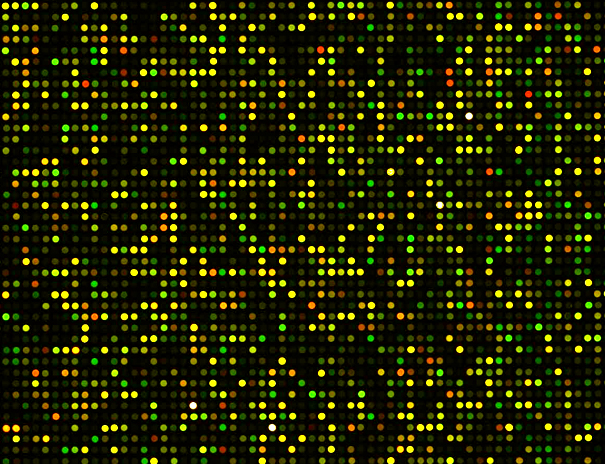
\includegraphics[width=.5\linewidth]{microarray.jpg}
  \end{center}
\end{frame}

\begin{frame}{Problems}
  \begin{itemize}
    \item High storage costs (memory)
    \item High computational costs (time)
    \item Visualization?
    \item Curse of dimensionality
  \end{itemize}
  \begin{center}
    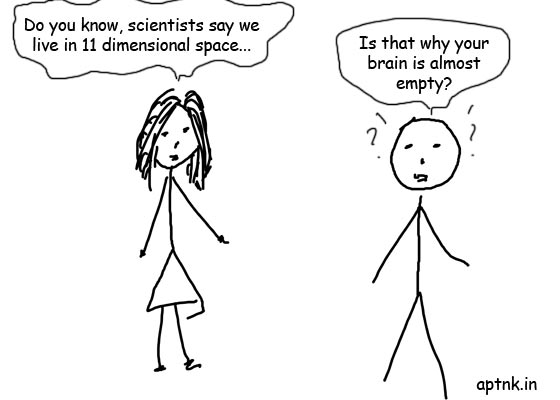
\includegraphics[width=.5\linewidth]{curse_dim.jpg}
  \end{center}
\end{frame}

\begin{frame}{Principle Component Analysis}
  \begin{itemize}
    \item Dimensionality reduction
    \item Visualization
    \item Missing values imputation
    \item Latent factors estimation:
      \begin{itemize}
        \item Population structure
        \item Batch-effects
        \item Cell-cycle
      \end{itemize}
  \end{itemize}
\end{frame}

\begin{frame}{Principle components}
  \begin{itemize}
    \item Minimize projection error
    \item Maximize variance
  \end{itemize}
  \begin{center}
    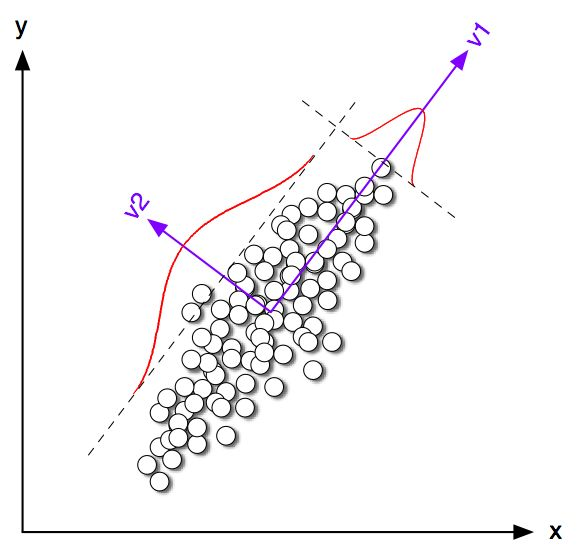
\includegraphics[width=.6\linewidth]{pca.jpg}
  \end{center}
\end{frame}

\begin{frame}{Pearson correlation coefficient}
  \begin{itemize}
    \item Measures \textbf{linear} dependency between $x$ and $y$
    \item $cor(x,y) = \in \left[-1,+1\right]$
    \item $cor(x,y) = 0$: no correlation
    \item $cor(x,y) = -1$: negative correlation
    \item $cor(x,y) = +1$: positive correlation
  \end{itemize}
  \begin{definition}[Pearson correlation coefficient]
    \begin{align*}
      \operatorname{cor}(x, y) = \frac{\sum_i (x_i - \bar{x})(y_i - \bar{y})}
      {\sqrt{\sum_i (x_i - \bar{x})^2}\sqrt{\sum_i (y_i - \bar{y})^2}}
    \end{align*}
  \end{definition}
\end{frame}

\begin{frame}{Pearson correlation coefficient}
  \begin{center}
    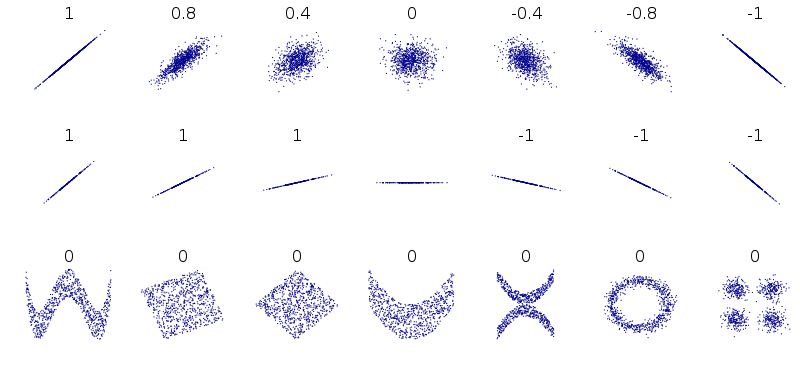
\includegraphics[width=0.8\linewidth]{pearson.png}
  \end{center}
\end{frame}

\begin{frame}{Spearman correlation coefficient}
  \begin{itemize}
    \item Measures \textbf{monotonic} dependency between $x$ and $y$
    \item Pearson correlation coefficient on rank of variables
    \item $cor(x,y) = \in \left[-1,+1\right]$
  \end{itemize}
  \begin{center}
    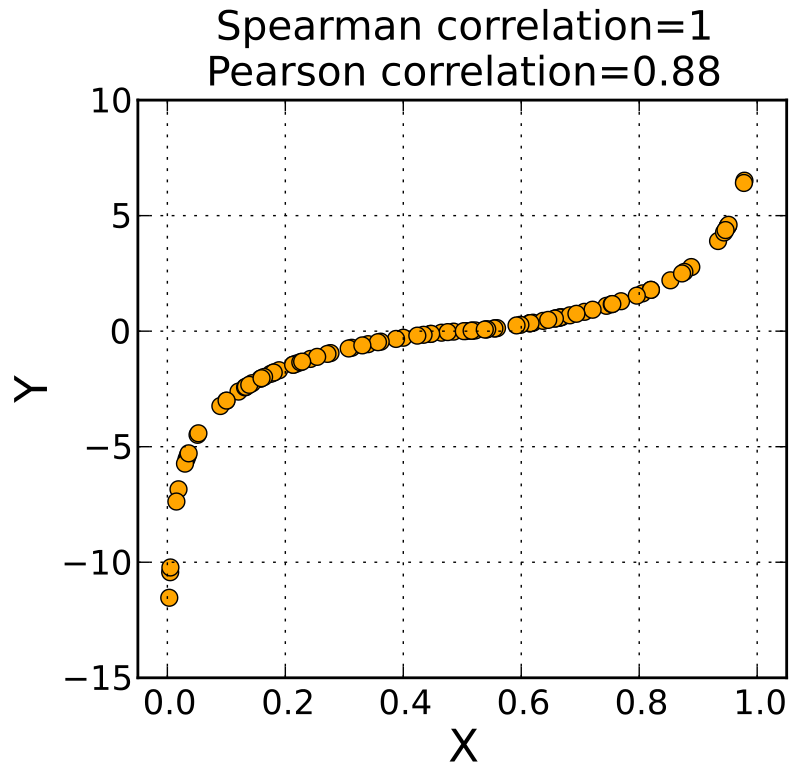
\includegraphics[width=0.4\linewidth]{spearman.png}
  \end{center}
\end{frame}



\begin{frame}[fragile]{ESC data}
  \begin{itemize}
    \item Single-cell RNA-seq
    \item $n=182$ Embryonic stem cells
    \item $p=9571$ Genes
    \item Cell-cycle via Hoechst staining
  \end{itemize}
\begin{knitrout}\tiny
\definecolor{shadecolor}{rgb}{0.969, 0.969, 0.969}\color{fgcolor}

{\centering \includegraphics[width=.9\linewidth]{figure/heat_esc} 

}


\begin{kframe}\begin{verbatim}
## [1]  182 9571
\end{verbatim}
\end{kframe}
\end{knitrout}
\end{frame}

\begin{frame}[fragile]{Correlation between two ESC}
\begin{knitrout}\tiny
\definecolor{shadecolor}{rgb}{0.969, 0.969, 0.969}\color{fgcolor}\begin{kframe}
\begin{alltt}
\hlstd{c1} \hlkwb{<-} \hlstd{esc}\hlopt{$}\hlstd{counts[}\hlkwd{which}\hlstd{(esc}\hlopt{$}\hlstd{cycle} \hlopt{==} \hlstr{'G1'}\hlstd{)[}\hlnum{1}\hlstd{],]}
\hlstd{c2} \hlkwb{<-} \hlstd{esc}\hlopt{$}\hlstd{counts[}\hlkwd{which}\hlstd{(esc}\hlopt{$}\hlstd{cycle} \hlopt{==} \hlstr{'S'}\hlstd{)[}\hlnum{1}\hlstd{],]}
\end{alltt}
\end{kframe}
\end{knitrout}
  \begin{columns}[c]
    \begin{column}{.5\linewidth}
\begin{knitrout}\tiny
\definecolor{shadecolor}{rgb}{0.969, 0.969, 0.969}\color{fgcolor}\begin{kframe}
\begin{alltt}
\hlkwd{qplot}\hlstd{(c1, c2,} \hlkwc{xlab}\hlstd{=}\hlstr{'G1 cell'}\hlstd{,} \hlkwc{ylab}\hlstd{=}\hlstr{'S cell'}\hlstd{)}
\end{alltt}
\end{kframe}

{\centering \includegraphics[width=\linewidth]{figure/cor_c1_c2} 

}



\end{knitrout}
    \end{column}
    \begin{column}{.5\linewidth}
\begin{knitrout}\tiny
\definecolor{shadecolor}{rgb}{0.969, 0.969, 0.969}\color{fgcolor}\begin{kframe}
\begin{alltt}
\hlkwd{cor}\hlstd{(c1, c2,}
    \hlkwc{method}\hlstd{=}\hlstr{'pearson'}\hlstd{)}
\end{alltt}
\begin{verbatim}
## [1] 0.5475
\end{verbatim}
\begin{alltt}
\hlkwd{cor}\hlstd{(c1, c2,}
    \hlkwc{method}\hlstd{=}\hlstr{'spearman'}\hlstd{)}
\end{alltt}
\begin{verbatim}
## [1] 0.5786
\end{verbatim}
\end{kframe}
\end{knitrout}
    \end{column}
  \end{columns}
\end{frame}

\begin{frame}[fragile]{Correlation matrix}
\begin{knitrout}\tiny
\definecolor{shadecolor}{rgb}{0.969, 0.969, 0.969}\color{fgcolor}\begin{kframe}
\begin{alltt}
\hlstd{cor_cells} \hlkwb{<-} \hlkwd{cor}\hlstd{(}\hlkwd{t}\hlstd{(esc}\hlopt{$}\hlstd{counts),} \hlkwc{method}\hlstd{=}\hlstr{'pearson'}\hlstd{)}
\hlkwd{heatmap}\hlstd{(cor_cells,} \hlkwc{Rowv}\hlstd{=}\hlnum{NA}\hlstd{,} \hlkwc{Colv}\hlstd{=}\hlnum{NA}\hlstd{)}
\end{alltt}
\end{kframe}

{\centering \includegraphics[width=.5\linewidth]{figure/cor_matrix} 

}



\end{knitrout}
\end{frame}

\begin{frame}[fragile]{PCA}
\begin{knitrout}\tiny
\definecolor{shadecolor}{rgb}{0.969, 0.969, 0.969}\color{fgcolor}\begin{kframe}
\begin{alltt}
\hlstd{svd} \hlkwb{<-} \hlkwd{svd}\hlstd{(}\hlkwd{scale}\hlstd{(esc}\hlopt{$}\hlstd{counts))}
\hlstd{dsvd} \hlkwb{<-} \hlkwd{as.data.frame}\hlstd{(svd}\hlopt{$}\hlstd{u[,} \hlnum{1}\hlopt{:}\hlnum{10}\hlstd{])}
\hlkwd{colnames}\hlstd{(dsvd)} \hlkwb{<-} \hlkwd{paste0}\hlstd{(}\hlstr{'pc'}\hlstd{,} \hlkwd{seq}\hlstd{(}\hlnum{1}\hlstd{,} \hlkwd{ncol}\hlstd{(dsvd)))}
\hlstd{dsvd}\hlopt{$}\hlstd{cycle} \hlkwb{<-} \hlstd{esc}\hlopt{$}\hlstd{cycle}
\hlstd{ve} \hlkwb{<-} \hlstd{svd}\hlopt{$}\hlstd{d}\hlopt{^}\hlnum{2} \hlopt{/} \hlkwd{sum}\hlstd{(svd}\hlopt{$}\hlstd{d}\hlopt{^}\hlnum{2}\hlstd{)}
\hlkwd{barplot}\hlstd{(ve[}\hlnum{1}\hlopt{:}\hlnum{10}\hlstd{],} \hlkwc{xlab}\hlstd{=}\hlstr{'Principle components'}\hlstd{,} \hlkwc{ylab}\hlstd{=}\hlstr{'% Variance explained'}\hlstd{,}
        \hlkwc{col}\hlstd{=}\hlstr{'lightblue'}\hlstd{)}
\end{alltt}
\end{kframe}

{\centering \includegraphics[width=.8\linewidth]{figure/pca_ve} 

}



\end{knitrout}
\end{frame}

\begin{frame}[fragile]{PC1 versus PC2}
\begin{knitrout}\tiny
\definecolor{shadecolor}{rgb}{0.969, 0.969, 0.969}\color{fgcolor}\begin{kframe}
\begin{alltt}
\hlkwd{ggplot}\hlstd{(dsvd,} \hlkwd{aes}\hlstd{(}\hlkwc{x}\hlstd{=pc1,} \hlkwc{y}\hlstd{=pc2,} \hlkwc{color}\hlstd{=cycle))} \hlopt{+} \hlkwd{geom_point}\hlstd{(}\hlkwc{size}\hlstd{=}\hlnum{3}\hlstd{)}
\end{alltt}
\end{kframe}

{\centering \includegraphics[width=.7\linewidth]{figure/pca_12} 

}



\end{knitrout}
\end{frame}

\begin{frame}[fragile]{Correlation PC1 and cell-cycle}
\begin{knitrout}\tiny
\definecolor{shadecolor}{rgb}{0.969, 0.969, 0.969}\color{fgcolor}\begin{kframe}
\begin{alltt}
\hlkwd{ggplot}\hlstd{(dsvd,} \hlkwd{aes}\hlstd{(}\hlkwc{x}\hlstd{=cycle,} \hlkwc{y}\hlstd{=pc1,} \hlkwc{color}\hlstd{=cycle))} \hlopt{+} \hlkwd{geom_boxplot}\hlstd{()} \hlopt{+} \hlkwd{geom_jitter}\hlstd{(}\hlkwc{position}\hlstd{=}\hlkwd{position_jitter}\hlstd{(}\hlkwc{width}\hlstd{=}\hlnum{.1}\hlstd{))}
\end{alltt}
\end{kframe}

{\centering \includegraphics[width=.7\linewidth]{figure/pca_cycle1} 

}



\end{knitrout}
\end{frame}

\begin{frame}[fragile]{Accounting for cell-cycle}
\begin{knitrout}\tiny
\definecolor{shadecolor}{rgb}{0.969, 0.969, 0.969}\color{fgcolor}\begin{kframe}
\begin{alltt}
\hlstd{svd_compress} \hlkwb{<-} \hlkwa{function}\hlstd{(}\hlkwc{svd}\hlstd{,} \hlkwc{k}\hlstd{=}\hlnum{1}\hlstd{) \{}
  \hlkwd{return} \hlstd{(svd}\hlopt{$}\hlstd{u[,} \hlnum{1}\hlopt{:}\hlstd{k,} \hlkwc{drop}\hlstd{=}\hlnum{FALSE}\hlstd{]} \hlopt \hlkwd{diag}\hlstd{(svd}\hlopt{$}\hlstd{d[}\hlnum{1}\hlopt{:}\hlstd{k],} \hlkwc{nrow}\hlstd{=k)} \hlopt \hlkwd{t}\hlstd{(svd}\hlopt{$}\hlstd{v)[}\hlnum{1}\hlopt{:}\hlstd{k,,} \hlkwc{drop}\hlstd{=}\hlnum{FALSE}\hlstd{])}
\hlstd{\}}
\hlstd{counts_pc1} \hlkwb{<-} \hlkwd{svd_compress}\hlstd{(svd,} \hlnum{1}\hlstd{)}
\hlstd{counts_npc1} \hlkwb{<-} \hlstd{esc}\hlopt{$}\hlstd{counts} \hlopt{-} \hlstd{counts_pc1}
\end{alltt}
\end{kframe}
\end{knitrout}
\end{frame}

\begin{frame}[fragile]{Raw counts}
\begin{knitrout}\tiny
\definecolor{shadecolor}{rgb}{0.969, 0.969, 0.969}\color{fgcolor}

{\centering \includegraphics[width=\linewidth]{figure/heat_esc2} 

}



\end{knitrout}
\end{frame}

\begin{frame}[fragile]{Counts explained by cell-cycle}
\begin{knitrout}\tiny
\definecolor{shadecolor}{rgb}{0.969, 0.969, 0.969}\color{fgcolor}

{\centering \includegraphics[width=\linewidth]{figure/heat_esc_pc1} 

}



\end{knitrout}
\end{frame}

\begin{frame}[fragile]{Counts after adjusting for cell-cycle}
\begin{knitrout}\tiny
\definecolor{shadecolor}{rgb}{0.969, 0.969, 0.969}\color{fgcolor}

{\centering \includegraphics[width=.9\linewidth]{figure/heat_esc_npc1} 

}



\end{knitrout}
\end{frame}


%knit_child('clust/main.Rnw')

\end{document}
